
%(BEGIN_QUESTION)
% Copyright 2015, Tony R. Kuphaldt, released under the Creative Commons Attribution License (v 1.0)
% This means you may do almost anything with this work of mine, so long as you give me proper credit

Magnetventil SV-92 har en viktig rolle i dette separator-kontrollsystemet på kompressorinntak. Nivåventil LV-92 åpner ved behov for å drenere væske fra ``boot''-delen av separatoren, som ideelt kun skal inneholde gass. Se P\&ID og svar:

$$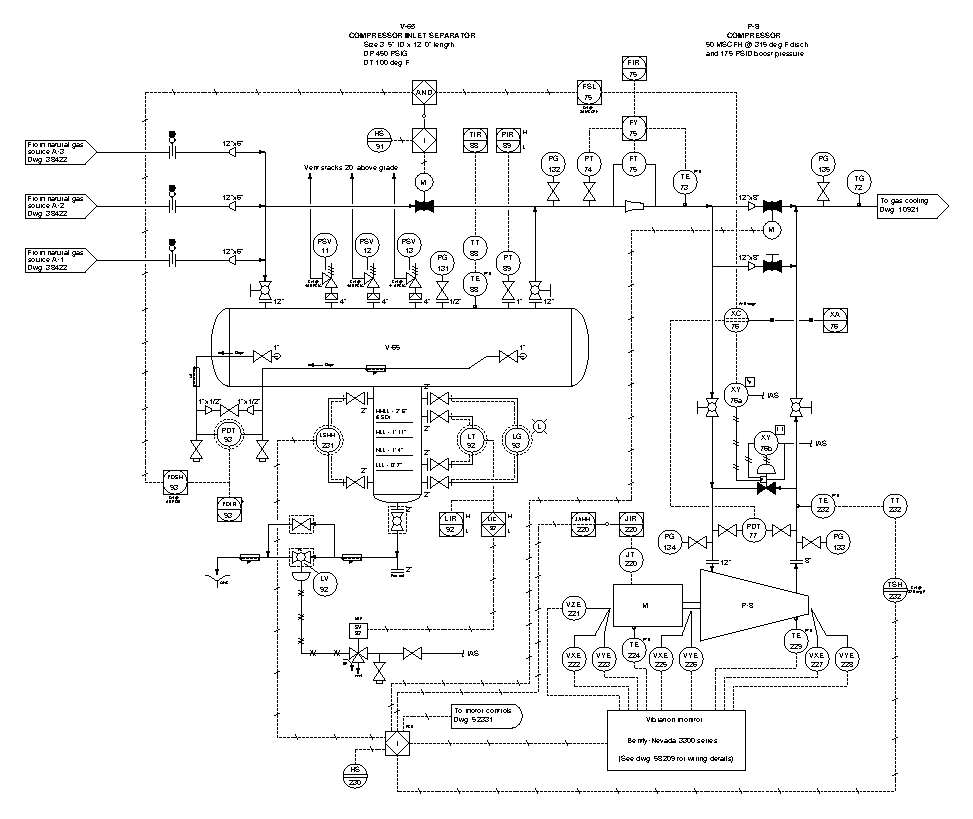
\includegraphics[width=15.5cm]{i0003rx01.eps}$$

\begin{itemize}
\item{} Angi status for SV-92 og LV-92 når væskenivå i separator-boot er ved eller under normalt nivå 1 fot 4 tommer.
\vskip 10pt
\item{} Beskriv hvordan systemet reagerer på høyt væskenivå i separator-boot.
\vskip 10pt
\item{} Hva blir konsekvensen av svikt i instrumentluftforsyning, relatert til væskenivå i boot?
\vskip 10pt
\item{} Hva blir konsekvensen av AC-strømsvikt til LIC-92?
\end{itemize}

\underbar{file i00953}
%(END_QUESTION)





%(BEGIN_ANSWER)

\begin{itemize}
\item{} Ved eller under normalnivå: {\it LV-92 er stengt, og spolen i SV-92 er spenningsløs.}
\vskip 10pt
\item{} Høyt nivå: {\it LT-92 måler høyt nivå, LIC-92 energiserer SV-92, luft sendes til aktuator på LV-92, og drainventilen åpner. Når nivået faller, de-energiseres SV-92 igjen.}
\vskip 10pt
\item{} Svikt i instrumentluft: {\it LV-92 kan ikke åpne, nivået stiger videre, og LSHH-231 vil til slutt trigge ESD for å stoppe kompressoren.}
\vskip 10pt
\item{} AC-svikt til LIC-92: {\it SV-92 kan ikke energiseres, LV-92 åpner ikke, nivået stiger videre, og LSHH-231 vil til slutt trigge ESD og stoppe kompressoren.}
\end{itemize}


%(END_ANSWER)





%(BEGIN_NOTES)


%INDEX% Final Control Elements, valve: fail-safe solenoids
%INDEX% Process: gas compressor inlet separator (realistic P&ID shown)

%(END_NOTES)

